\documentclass[]{book}
\usepackage{lmodern}
\usepackage{amssymb,amsmath}
\usepackage{ifxetex,ifluatex}
\usepackage{fixltx2e} % provides \textsubscript
\ifnum 0\ifxetex 1\fi\ifluatex 1\fi=0 % if pdftex
  \usepackage[T1]{fontenc}
  \usepackage[utf8]{inputenc}
\else % if luatex or xelatex
  \ifxetex
    \usepackage{mathspec}
  \else
    \usepackage{fontspec}
  \fi
  \defaultfontfeatures{Ligatures=TeX,Scale=MatchLowercase}
\fi
% use upquote if available, for straight quotes in verbatim environments
\IfFileExists{upquote.sty}{\usepackage{upquote}}{}
% use microtype if available
\IfFileExists{microtype.sty}{%
\usepackage{microtype}
\UseMicrotypeSet[protrusion]{basicmath} % disable protrusion for tt fonts
}{}
\usepackage{hyperref}
\hypersetup{unicode=true,
            pdftitle={Intro To dplyr},
            pdfauthor={Steve Pittard},
            pdfborder={0 0 0},
            breaklinks=true}
\urlstyle{same}  % don't use monospace font for urls
\usepackage{natbib}
\bibliographystyle{apalike}
\usepackage{color}
\usepackage{fancyvrb}
\newcommand{\VerbBar}{|}
\newcommand{\VERB}{\Verb[commandchars=\\\{\}]}
\DefineVerbatimEnvironment{Highlighting}{Verbatim}{commandchars=\\\{\}}
% Add ',fontsize=\small' for more characters per line
\usepackage{framed}
\definecolor{shadecolor}{RGB}{248,248,248}
\newenvironment{Shaded}{\begin{snugshade}}{\end{snugshade}}
\newcommand{\KeywordTok}[1]{\textcolor[rgb]{0.13,0.29,0.53}{\textbf{#1}}}
\newcommand{\DataTypeTok}[1]{\textcolor[rgb]{0.13,0.29,0.53}{#1}}
\newcommand{\DecValTok}[1]{\textcolor[rgb]{0.00,0.00,0.81}{#1}}
\newcommand{\BaseNTok}[1]{\textcolor[rgb]{0.00,0.00,0.81}{#1}}
\newcommand{\FloatTok}[1]{\textcolor[rgb]{0.00,0.00,0.81}{#1}}
\newcommand{\ConstantTok}[1]{\textcolor[rgb]{0.00,0.00,0.00}{#1}}
\newcommand{\CharTok}[1]{\textcolor[rgb]{0.31,0.60,0.02}{#1}}
\newcommand{\SpecialCharTok}[1]{\textcolor[rgb]{0.00,0.00,0.00}{#1}}
\newcommand{\StringTok}[1]{\textcolor[rgb]{0.31,0.60,0.02}{#1}}
\newcommand{\VerbatimStringTok}[1]{\textcolor[rgb]{0.31,0.60,0.02}{#1}}
\newcommand{\SpecialStringTok}[1]{\textcolor[rgb]{0.31,0.60,0.02}{#1}}
\newcommand{\ImportTok}[1]{#1}
\newcommand{\CommentTok}[1]{\textcolor[rgb]{0.56,0.35,0.01}{\textit{#1}}}
\newcommand{\DocumentationTok}[1]{\textcolor[rgb]{0.56,0.35,0.01}{\textbf{\textit{#1}}}}
\newcommand{\AnnotationTok}[1]{\textcolor[rgb]{0.56,0.35,0.01}{\textbf{\textit{#1}}}}
\newcommand{\CommentVarTok}[1]{\textcolor[rgb]{0.56,0.35,0.01}{\textbf{\textit{#1}}}}
\newcommand{\OtherTok}[1]{\textcolor[rgb]{0.56,0.35,0.01}{#1}}
\newcommand{\FunctionTok}[1]{\textcolor[rgb]{0.00,0.00,0.00}{#1}}
\newcommand{\VariableTok}[1]{\textcolor[rgb]{0.00,0.00,0.00}{#1}}
\newcommand{\ControlFlowTok}[1]{\textcolor[rgb]{0.13,0.29,0.53}{\textbf{#1}}}
\newcommand{\OperatorTok}[1]{\textcolor[rgb]{0.81,0.36,0.00}{\textbf{#1}}}
\newcommand{\BuiltInTok}[1]{#1}
\newcommand{\ExtensionTok}[1]{#1}
\newcommand{\PreprocessorTok}[1]{\textcolor[rgb]{0.56,0.35,0.01}{\textit{#1}}}
\newcommand{\AttributeTok}[1]{\textcolor[rgb]{0.77,0.63,0.00}{#1}}
\newcommand{\RegionMarkerTok}[1]{#1}
\newcommand{\InformationTok}[1]{\textcolor[rgb]{0.56,0.35,0.01}{\textbf{\textit{#1}}}}
\newcommand{\WarningTok}[1]{\textcolor[rgb]{0.56,0.35,0.01}{\textbf{\textit{#1}}}}
\newcommand{\AlertTok}[1]{\textcolor[rgb]{0.94,0.16,0.16}{#1}}
\newcommand{\ErrorTok}[1]{\textcolor[rgb]{0.64,0.00,0.00}{\textbf{#1}}}
\newcommand{\NormalTok}[1]{#1}
\usepackage{longtable,booktabs}
\usepackage{graphicx,grffile}
\makeatletter
\def\maxwidth{\ifdim\Gin@nat@width>\linewidth\linewidth\else\Gin@nat@width\fi}
\def\maxheight{\ifdim\Gin@nat@height>\textheight\textheight\else\Gin@nat@height\fi}
\makeatother
% Scale images if necessary, so that they will not overflow the page
% margins by default, and it is still possible to overwrite the defaults
% using explicit options in \includegraphics[width, height, ...]{}
\setkeys{Gin}{width=\maxwidth,height=\maxheight,keepaspectratio}
\IfFileExists{parskip.sty}{%
\usepackage{parskip}
}{% else
\setlength{\parindent}{0pt}
\setlength{\parskip}{6pt plus 2pt minus 1pt}
}
\setlength{\emergencystretch}{3em}  % prevent overfull lines
\providecommand{\tightlist}{%
  \setlength{\itemsep}{0pt}\setlength{\parskip}{0pt}}
\setcounter{secnumdepth}{5}
% Redefines (sub)paragraphs to behave more like sections
\ifx\paragraph\undefined\else
\let\oldparagraph\paragraph
\renewcommand{\paragraph}[1]{\oldparagraph{#1}\mbox{}}
\fi
\ifx\subparagraph\undefined\else
\let\oldsubparagraph\subparagraph
\renewcommand{\subparagraph}[1]{\oldsubparagraph{#1}\mbox{}}
\fi

%%% Use protect on footnotes to avoid problems with footnotes in titles
\let\rmarkdownfootnote\footnote%
\def\footnote{\protect\rmarkdownfootnote}

%%% Change title format to be more compact
\usepackage{titling}

% Create subtitle command for use in maketitle
\providecommand{\subtitle}[1]{
  \posttitle{
    \begin{center}\large#1\end{center}
    }
}

\setlength{\droptitle}{-2em}

  \title{Intro To dplyr}
    \pretitle{\vspace{\droptitle}\centering\huge}
  \posttitle{\par}
    \author{Steve Pittard}
    \preauthor{\centering\large\emph}
  \postauthor{\par}
      \predate{\centering\large\emph}
  \postdate{\par}
    \date{2020-01-24}

\usepackage{booktabs}

\begin{document}
\maketitle

{
\setcounter{tocdepth}{1}
\tableofcontents
}
\chapter{R Data Structures}\label{r-data-structures}

There are a number of data structures in R such as \textbf{vectors,
lists, matricies} and \textbf{arrays} but the the premier data structure
in R is known as the \textbf{data.frame}. This structure can be
described as follows:

\begin{itemize}
\item
  A data frame is a special type of list that contains data in a format
  that allows for easier manipulation, reshaping, and open-ended
  analysis
\item
  Data frames are tightly coupled collections of variables. It is one of
  the more important constructs you will encounter when using R so learn
  all you can about it
\item
  A data frame is an analogue to the Excel spreadsheet but is much more
  flexible for storing, manipulating, and analyzing data
\item
  Data frames can be constructed from existing vectors, lists, or
  matrices. Many times they are created by reading in comma delimited
  files, (CSV files), using the read.table command
\end{itemize}

Once you become accustomed to working with data frames, R becomes so
much easier to use. In fact, it could be well argued tht UNTIL you wrap
your head around the data frame concept then you cannot be productive in
R. This is mostly true, in my experience.

\section{The Mighty Data Frame}\label{the-mighty-data-frame}

\begin{figure}
\centering
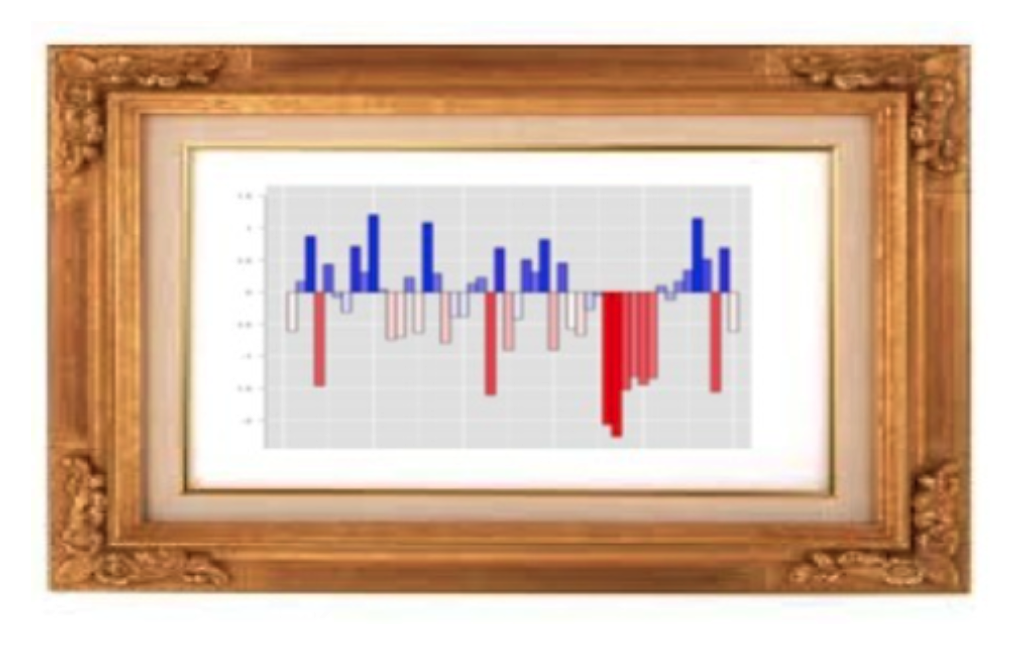
\includegraphics[width=3.12500in]{./figures/dframe.png}
\caption{}
\end{figure}

R comes with with a variety of built-in data sets that are very useful
for getting used to data sets and how to manipulate them.

\begin{Shaded}
\begin{Highlighting}[]
\NormalTok{AirPassengers           Monthly Airline Passenger Numbers }\DecValTok{1949}\OperatorTok{-}\DecValTok{1960}
\NormalTok{BJsales                 Sales Data with Leading Indicator}
\NormalTok{BOD                     Biochemical Oxygen Demand}
\NormalTok{CO2                     Carbon Dioxide Uptake }\ControlFlowTok{in}\NormalTok{ Grass Plants}
\NormalTok{ChickWeight             Weight versus age of chicks on different diets}
\NormalTok{DNase                   Elisa assay of DNase}
\NormalTok{Formaldehyde            Determination of Formaldehyde}
\NormalTok{HairEyeColor            Hair and Eye Color of Statistics Students}
\NormalTok{Harman23.cor            Harman Example }\FloatTok{2.3}
\NormalTok{Harman74.cor            Harman Example }\FloatTok{7.4}
\NormalTok{Indometh                Pharmacokinetics of Indomethacin}
\NormalTok{InsectSprays            Effectiveness of Insect Sprays}
\NormalTok{JohnsonJohnson          Quarterly Earnings per Johnson }\OperatorTok{&}\StringTok{ }\NormalTok{Johnson Share}
\NormalTok{LakeHuron               Level of Lake Huron }\DecValTok{1875}\OperatorTok{-}\DecValTok{1972}
\NormalTok{LifeCycleSavings        Intercountry Life}\OperatorTok{-}\NormalTok{Cycle Savings Data}
\NormalTok{Loblolly                Growth of Loblolly pine trees}
\NormalTok{Nile                    Flow of the River Nile}
\NormalTok{Orange                  Growth of Orange Trees}
\NormalTok{OrchardSprays           Potency of Orchard Sprays}
\NormalTok{PlantGrowth             Results from an Experiment on Plant Growth}
\NormalTok{Puromycin               Reaction Velocity of an Enzymatic Reaction}
\NormalTok{Theoph                  Pharmacokinetics of Theophylline}
\end{Highlighting}
\end{Shaded}

\section{A Reference Data Frame}\label{a-reference-data-frame}

We will use a well-known data frame, at least in R circles, called
\textbf{mtcars} which is part of any default installation of R. It is a
simple data set relating to, well, automobiles. This data frame has the
distinction of being the most (ab)used data frame in R education.

\begin{Shaded}
\begin{Highlighting}[]
\NormalTok{The data was extracted from the }\DecValTok{1974}\NormalTok{ Motor Trend US }
\NormalTok{magazine, and comprises fuel consumption and }\DecValTok{10}\NormalTok{ aspects }
\NormalTok{of automobile design and performance }\ControlFlowTok{for} \DecValTok{32}\NormalTok{ automobiles }
\NormalTok{(}\DecValTok{1973}\NormalTok{–}\DecValTok{74}\NormalTok{ models).}

\NormalTok{A data frame with }\DecValTok{32}\NormalTok{ observations on }\DecValTok{11}\NormalTok{ (numeric) }
\NormalTok{variables.}

\NormalTok{[, }\DecValTok{1}\NormalTok{]   mpg Miles}\OperatorTok{/}\NormalTok{(US) gallon}
\NormalTok{[, }\DecValTok{2}\NormalTok{]   cyl Number of cylinders}
\NormalTok{[, }\DecValTok{3}\NormalTok{]   disp    }\KeywordTok{Displacement}\NormalTok{ (cu.in.)}
\NormalTok{[, }\DecValTok{4}\NormalTok{]   hp  Gross horsepower}
\NormalTok{[, }\DecValTok{5}\NormalTok{]   drat    Rear axle ratio}
\NormalTok{[, }\DecValTok{6}\NormalTok{]   wt  }\KeywordTok{Weight}\NormalTok{ (}\DecValTok{1000}\NormalTok{ lbs)}
\NormalTok{[, }\DecValTok{7}\NormalTok{]   qsec    }\DecValTok{1}\OperatorTok{/}\DecValTok{4}\NormalTok{ mile time}
\NormalTok{[, }\DecValTok{8}\NormalTok{]   vs  }\KeywordTok{Engine}\NormalTok{ (}\DecValTok{0}\NormalTok{ =}\StringTok{ }\NormalTok{V}\OperatorTok{-}\NormalTok{shaped, }\DecValTok{1}\NormalTok{ =}\StringTok{ }\NormalTok{straight)}
\NormalTok{[, }\DecValTok{9}\NormalTok{]   am  }\KeywordTok{Transmission}\NormalTok{ (}\DecValTok{0}\NormalTok{ =}\StringTok{ }\NormalTok{automatic, }\DecValTok{1}\NormalTok{ =}\StringTok{ }\NormalTok{manual)}
\NormalTok{[,}\DecValTok{10}\NormalTok{]   gear    Number of forward gears}
\NormalTok{[,}\DecValTok{11}\NormalTok{]   carb    Number of carburetors}
\end{Highlighting}
\end{Shaded}

\section{Relation to dplyr}\label{relation-to-dplyr}

What you will discover is that the \textbf{dplyr} package, which itself
is part of the much larger \textbf{tidyverse} package set , extends upon
the idea of the basic R data frame in a way that some feel is superior.
It depends on your point of view though the \textbf{tidyverse} has a lot
of what I call a philosophic consistency in it which makes it
\textbf{very} useful once you get some concepts in mind.

While you could start exclusively with \textbf{dplyr} and the
\textbf{tidyverse} the world is still full of older code. Plus, many of
the advantages of \textbf{dplyr} only become quite apparent when
compared to the ``older way'' of doing things. So my recommendation is
to know how to deal with data frames in base R while also spending time
to learn the \textbf{dplyr} way of doing things.

\chapter{An Example}\label{an-example}

Data frames look like an Excel Spreadsheet. The rows are observations
and the columns are variables or ``features'' that represent some
measurement or character-based description of a given observation. When
viewed from the row point of view, the data can be heterogenous. When
viewed as a column, the data is homogenous.

\begin{Shaded}
\begin{Highlighting}[]
\KeywordTok{data}\NormalTok{(mtcars)}
\NormalTok{mtcars}
\end{Highlighting}
\end{Shaded}

\begin{verbatim}
##                      mpg cyl  disp  hp drat    wt  qsec vs am gear carb
## Mazda RX4           21.0   6 160.0 110 3.90 2.620 16.46  0  1    4    4
## Mazda RX4 Wag       21.0   6 160.0 110 3.90 2.875 17.02  0  1    4    4
## Datsun 710          22.8   4 108.0  93 3.85 2.320 18.61  1  1    4    1
## Hornet 4 Drive      21.4   6 258.0 110 3.08 3.215 19.44  1  0    3    1
## Hornet Sportabout   18.7   8 360.0 175 3.15 3.440 17.02  0  0    3    2
## Valiant             18.1   6 225.0 105 2.76 3.460 20.22  1  0    3    1
## Duster 360          14.3   8 360.0 245 3.21 3.570 15.84  0  0    3    4
## Merc 240D           24.4   4 146.7  62 3.69 3.190 20.00  1  0    4    2
## Merc 230            22.8   4 140.8  95 3.92 3.150 22.90  1  0    4    2
## Merc 280            19.2   6 167.6 123 3.92 3.440 18.30  1  0    4    4
## Merc 280C           17.8   6 167.6 123 3.92 3.440 18.90  1  0    4    4
## Merc 450SE          16.4   8 275.8 180 3.07 4.070 17.40  0  0    3    3
## Merc 450SL          17.3   8 275.8 180 3.07 3.730 17.60  0  0    3    3
## Merc 450SLC         15.2   8 275.8 180 3.07 3.780 18.00  0  0    3    3
## Cadillac Fleetwood  10.4   8 472.0 205 2.93 5.250 17.98  0  0    3    4
## Lincoln Continental 10.4   8 460.0 215 3.00 5.424 17.82  0  0    3    4
## Chrysler Imperial   14.7   8 440.0 230 3.23 5.345 17.42  0  0    3    4
## Fiat 128            32.4   4  78.7  66 4.08 2.200 19.47  1  1    4    1
## Honda Civic         30.4   4  75.7  52 4.93 1.615 18.52  1  1    4    2
## Toyota Corolla      33.9   4  71.1  65 4.22 1.835 19.90  1  1    4    1
## Toyota Corona       21.5   4 120.1  97 3.70 2.465 20.01  1  0    3    1
## Dodge Challenger    15.5   8 318.0 150 2.76 3.520 16.87  0  0    3    2
## AMC Javelin         15.2   8 304.0 150 3.15 3.435 17.30  0  0    3    2
## Camaro Z28          13.3   8 350.0 245 3.73 3.840 15.41  0  0    3    4
## Pontiac Firebird    19.2   8 400.0 175 3.08 3.845 17.05  0  0    3    2
## Fiat X1-9           27.3   4  79.0  66 4.08 1.935 18.90  1  1    4    1
## Porsche 914-2       26.0   4 120.3  91 4.43 2.140 16.70  0  1    5    2
## Lotus Europa        30.4   4  95.1 113 3.77 1.513 16.90  1  1    5    2
## Ford Pantera L      15.8   8 351.0 264 4.22 3.170 14.50  0  1    5    4
## Ferrari Dino        19.7   6 145.0 175 3.62 2.770 15.50  0  1    5    6
## Maserati Bora       15.0   8 301.0 335 3.54 3.570 14.60  0  1    5    8
## Volvo 142E          21.4   4 121.0 109 4.11 2.780 18.60  1  1    4    2
\end{verbatim}

We can do this with this data such as make plots or create models:

\begin{Shaded}
\begin{Highlighting}[]
\KeywordTok{plot}\NormalTok{(mpg }\OperatorTok{~}\StringTok{ }\NormalTok{wt, }\DataTypeTok{data=}\NormalTok{mtcars)}
\end{Highlighting}
\end{Shaded}

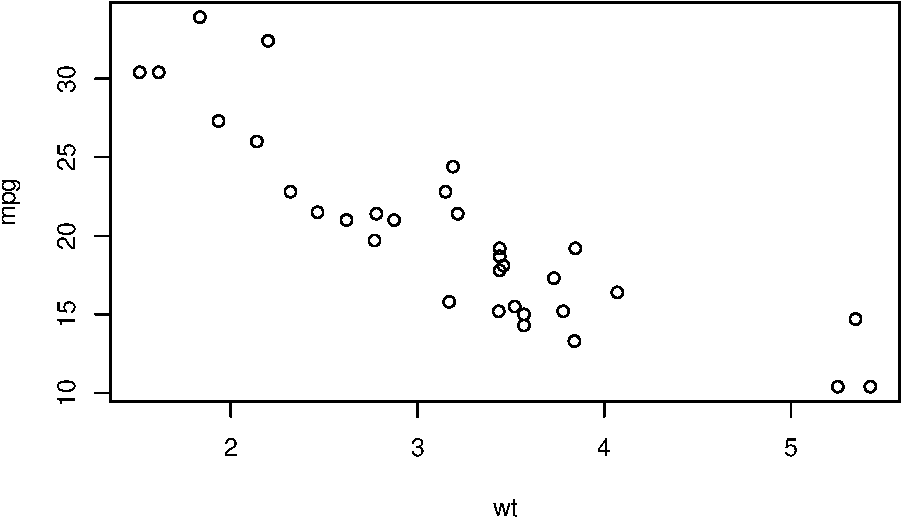
\includegraphics{nursing_741_files/figure-latex/cars-1.pdf}

Let's create a regression model. It doesn't take long to realize that
most functions in R will use a data frame as input. This means that you
will spend a lot of time working with data frames to get them into shape
for use with modeling and visualization tools. In fact you will spend
most of your time \textbf{importing, transforming, and cleaning}.

\begin{Shaded}
\begin{Highlighting}[]
\NormalTok{(mylm <-}\StringTok{ }\KeywordTok{lm}\NormalTok{(mpg }\OperatorTok{~}\StringTok{ }\NormalTok{., }\DataTypeTok{data =}\NormalTok{ mtcars))}
\end{Highlighting}
\end{Shaded}

\begin{verbatim}
## 
## Call:
## lm(formula = mpg ~ ., data = mtcars)
## 
## Coefficients:
## (Intercept)          cyl         disp           hp         drat  
##    12.30337     -0.11144      0.01334     -0.02148      0.78711  
##          wt         qsec           vs           am         gear  
##    -3.71530      0.82104      0.31776      2.52023      0.65541  
##        carb  
##    -0.19942
\end{verbatim}

There are some useful functions that help you understand the structure
of a data frame. One of the most important ones is called the
\textbf{str()} function which is short hand for \textbf{structure}.

\section{Structure}\label{structure}

\begin{Shaded}
\begin{Highlighting}[]
\KeywordTok{str}\NormalTok{(mtcars)}
\end{Highlighting}
\end{Shaded}

\begin{verbatim}
## 'data.frame':    32 obs. of  11 variables:
##  $ mpg : num  21 21 22.8 21.4 18.7 18.1 14.3 24.4 22.8 19.2 ...
##  $ cyl : num  6 6 4 6 8 6 8 4 4 6 ...
##  $ disp: num  160 160 108 258 360 ...
##  $ hp  : num  110 110 93 110 175 105 245 62 95 123 ...
##  $ drat: num  3.9 3.9 3.85 3.08 3.15 2.76 3.21 3.69 3.92 3.92 ...
##  $ wt  : num  2.62 2.88 2.32 3.21 3.44 ...
##  $ qsec: num  16.5 17 18.6 19.4 17 ...
##  $ vs  : num  0 0 1 1 0 1 0 1 1 1 ...
##  $ am  : num  1 1 1 0 0 0 0 0 0 0 ...
##  $ gear: num  4 4 4 3 3 3 3 4 4 4 ...
##  $ carb: num  4 4 1 1 2 1 4 2 2 4 ...
\end{verbatim}

This gives you some idea about the number of rows and columns of the
data frame along with a description of the variable types and their
values. I use this function frequently. Other functions that will help
you include the following.

\section{Meta Information}\label{meta-information}

\begin{Shaded}
\begin{Highlighting}[]
\CommentTok{# how many rows}
\KeywordTok{nrow}\NormalTok{(mtcars) }
\end{Highlighting}
\end{Shaded}

\begin{verbatim}
## [1] 32
\end{verbatim}

\begin{Shaded}
\begin{Highlighting}[]
\CommentTok{# how many columns}
\KeywordTok{ncol}\NormalTok{(mtcars) }
\end{Highlighting}
\end{Shaded}

\begin{verbatim}
## [1] 11
\end{verbatim}

\begin{Shaded}
\begin{Highlighting}[]
\CommentTok{# Column names}
\KeywordTok{names}\NormalTok{(mtcars)}
\end{Highlighting}
\end{Shaded}

\begin{verbatim}
##  [1] "mpg"  "cyl"  "disp" "hp"   "drat" "wt"   "qsec" "vs"   "am"   "gear"
## [11] "carb"
\end{verbatim}

\section{Printing}\label{printing}

Some data frames, such as mtcars, don't have many rows but others might
have hundreds, thousands or even more than that ! Imagine trying to view
one of those data frames. It is for this reason that the \textbf{head()}
and \textbf{tail()} functions exist.

\begin{Shaded}
\begin{Highlighting}[]
\KeywordTok{head}\NormalTok{(mtcars,}\DecValTok{5}\NormalTok{) }\CommentTok{# First 5 rows}
\end{Highlighting}
\end{Shaded}

\begin{verbatim}
##                    mpg cyl disp  hp drat    wt  qsec vs am gear carb
## Mazda RX4         21.0   6  160 110 3.90 2.620 16.46  0  1    4    4
## Mazda RX4 Wag     21.0   6  160 110 3.90 2.875 17.02  0  1    4    4
## Datsun 710        22.8   4  108  93 3.85 2.320 18.61  1  1    4    1
## Hornet 4 Drive    21.4   6  258 110 3.08 3.215 19.44  1  0    3    1
## Hornet Sportabout 18.7   8  360 175 3.15 3.440 17.02  0  0    3    2
\end{verbatim}

\begin{Shaded}
\begin{Highlighting}[]
\KeywordTok{tail}\NormalTok{(mtcars,}\DecValTok{3}\NormalTok{) }\CommentTok{# Last 3 rows}
\end{Highlighting}
\end{Shaded}

\begin{verbatim}
##                mpg cyl disp  hp drat   wt qsec vs am gear carb
## Ferrari Dino  19.7   6  145 175 3.62 2.77 15.5  0  1    5    6
## Maserati Bora 15.0   8  301 335 3.54 3.57 14.6  0  1    5    8
## Volvo 142E    21.4   4  121 109 4.11 2.78 18.6  1  1    4    2
\end{verbatim}

\section{Accessing Rows And Columns}\label{accessing-rows-and-columns}

There are various ways to select, remove, or exclude rows and columns of
a data frame. We use the \textbf{bracket} notation to do this. This is
very powerful. Keep in mind that data frames have rows and columns so it
would make sense that you need a way to specify what rows and columns
you want to access.

\begin{Shaded}
\begin{Highlighting}[]
\NormalTok{mtcars[}\DecValTok{1}\NormalTok{,]     }\CommentTok{# First row, all columns}
\end{Highlighting}
\end{Shaded}

\begin{verbatim}
##           mpg cyl disp  hp drat   wt  qsec vs am gear carb
## Mazda RX4  21   6  160 110  3.9 2.62 16.46  0  1    4    4
\end{verbatim}

\begin{Shaded}
\begin{Highlighting}[]
\NormalTok{mtcars[}\DecValTok{1}\OperatorTok{:}\DecValTok{3}\NormalTok{,]   }\CommentTok{# First three rows, all columns}
\end{Highlighting}
\end{Shaded}

\begin{verbatim}
##                mpg cyl disp  hp drat    wt  qsec vs am gear carb
## Mazda RX4     21.0   6  160 110 3.90 2.620 16.46  0  1    4    4
## Mazda RX4 Wag 21.0   6  160 110 3.90 2.875 17.02  0  1    4    4
## Datsun 710    22.8   4  108  93 3.85 2.320 18.61  1  1    4    1
\end{verbatim}

\begin{Shaded}
\begin{Highlighting}[]
\CommentTok{# All rows, and first 4 columns}
\NormalTok{mtcars[,}\DecValTok{1}\OperatorTok{:}\DecValTok{4}\NormalTok{]   }
\end{Highlighting}
\end{Shaded}

\begin{verbatim}
##                      mpg cyl  disp  hp
## Mazda RX4           21.0   6 160.0 110
## Mazda RX4 Wag       21.0   6 160.0 110
## Datsun 710          22.8   4 108.0  93
## Hornet 4 Drive      21.4   6 258.0 110
## Hornet Sportabout   18.7   8 360.0 175
## Valiant             18.1   6 225.0 105
## Duster 360          14.3   8 360.0 245
## Merc 240D           24.4   4 146.7  62
## Merc 230            22.8   4 140.8  95
## Merc 280            19.2   6 167.6 123
## Merc 280C           17.8   6 167.6 123
## Merc 450SE          16.4   8 275.8 180
## Merc 450SL          17.3   8 275.8 180
## Merc 450SLC         15.2   8 275.8 180
## Cadillac Fleetwood  10.4   8 472.0 205
## Lincoln Continental 10.4   8 460.0 215
## Chrysler Imperial   14.7   8 440.0 230
## Fiat 128            32.4   4  78.7  66
## Honda Civic         30.4   4  75.7  52
## Toyota Corolla      33.9   4  71.1  65
## Toyota Corona       21.5   4 120.1  97
## Dodge Challenger    15.5   8 318.0 150
## AMC Javelin         15.2   8 304.0 150
## Camaro Z28          13.3   8 350.0 245
## Pontiac Firebird    19.2   8 400.0 175
## Fiat X1-9           27.3   4  79.0  66
## Porsche 914-2       26.0   4 120.3  91
## Lotus Europa        30.4   4  95.1 113
## Ford Pantera L      15.8   8 351.0 264
## Ferrari Dino        19.7   6 145.0 175
## Maserati Bora       15.0   8 301.0 335
## Volvo 142E          21.4   4 121.0 109
\end{verbatim}

\begin{Shaded}
\begin{Highlighting}[]
\CommentTok{# Rows 1-5 and columns 1,2 and 8-10}
\NormalTok{mtcars[}\DecValTok{1}\OperatorTok{:}\DecValTok{4}\NormalTok{,}\KeywordTok{c}\NormalTok{(}\DecValTok{1}\OperatorTok{:}\DecValTok{2}\NormalTok{,}\DecValTok{8}\OperatorTok{:}\DecValTok{10}\NormalTok{)]}
\end{Highlighting}
\end{Shaded}

\begin{verbatim}
##                 mpg cyl vs am gear
## Mazda RX4      21.0   6  0  1    4
## Mazda RX4 Wag  21.0   6  0  1    4
## Datsun 710     22.8   4  1  1    4
## Hornet 4 Drive 21.4   6  1  0    3
\end{verbatim}

\begin{Shaded}
\begin{Highlighting}[]
\CommentTok{# Rows 1-5 and columns 1,2 and 8-10}
\NormalTok{mtcars[}\DecValTok{1}\OperatorTok{:}\DecValTok{4}\NormalTok{,}\KeywordTok{c}\NormalTok{(}\DecValTok{1}\OperatorTok{:}\DecValTok{2}\NormalTok{,}\DecValTok{8}\OperatorTok{:}\DecValTok{10}\NormalTok{)]}
\end{Highlighting}
\end{Shaded}

\begin{verbatim}
##                 mpg cyl vs am gear
## Mazda RX4      21.0   6  0  1    4
## Mazda RX4 Wag  21.0   6  0  1    4
## Datsun 710     22.8   4  1  1    4
## Hornet 4 Drive 21.4   6  1  0    3
\end{verbatim}

\begin{Shaded}
\begin{Highlighting}[]
\CommentTok{# Rows 1-5 and columns by name}
\NormalTok{mtcars[}\DecValTok{1}\OperatorTok{:}\DecValTok{4}\NormalTok{,}\KeywordTok{c}\NormalTok{(}\StringTok{"mpg"}\NormalTok{,}\StringTok{"wt"}\NormalTok{,}\StringTok{"drat"}\NormalTok{)]}
\end{Highlighting}
\end{Shaded}

\begin{verbatim}
##                 mpg    wt drat
## Mazda RX4      21.0 2.620 3.90
## Mazda RX4 Wag  21.0 2.875 3.90
## Datsun 710     22.8 2.320 3.85
## Hornet 4 Drive 21.4 3.215 3.08
\end{verbatim}

\section{Interrogating}\label{interrogating}

Many times you will wish to find rows that satisfy certain conditions.
For example, what rows have an mpg \textgreater{} 11 and at wt
\textless{} 2.0 ? We use the bracket notation to help us. We can pass
logical conditions into the brackets. Note the following:

\begin{Shaded}
\begin{Highlighting}[]
\NormalTok{mtcars}\OperatorTok{$}\NormalTok{mpg }\OperatorTok{>}\StringTok{ }\DecValTok{11} \OperatorTok{&}\StringTok{ }\NormalTok{mtcars}\OperatorTok{$}\NormalTok{wt }\OperatorTok{<}\StringTok{ }\FloatTok{2.0}
\end{Highlighting}
\end{Shaded}

\begin{verbatim}
##  [1] FALSE FALSE FALSE FALSE FALSE FALSE FALSE FALSE FALSE FALSE FALSE
## [12] FALSE FALSE FALSE FALSE FALSE FALSE FALSE  TRUE  TRUE FALSE FALSE
## [23] FALSE FALSE FALSE  TRUE FALSE  TRUE FALSE FALSE FALSE FALSE
\end{verbatim}

There are 32 elements in this logical vector each with a value of either
TRUE or FALSE. When passed into the row index of the bracket notation,
it will print that row if the corresponding value is TRUE. If FALSE, the
row will not be printed.

\begin{Shaded}
\begin{Highlighting}[]
\NormalTok{mtcars[mtcars}\OperatorTok{$}\NormalTok{mpg }\OperatorTok{>}\StringTok{ }\DecValTok{11} \OperatorTok{&}\StringTok{ }\NormalTok{mtcars}\OperatorTok{$}\NormalTok{wt }\OperatorTok{<}\StringTok{ }\FloatTok{2.0}\NormalTok{,]}
\end{Highlighting}
\end{Shaded}

\begin{verbatim}
##                 mpg cyl disp  hp drat    wt  qsec vs am gear carb
## Honda Civic    30.4   4 75.7  52 4.93 1.615 18.52  1  1    4    2
## Toyota Corolla 33.9   4 71.1  65 4.22 1.835 19.90  1  1    4    1
## Fiat X1-9      27.3   4 79.0  66 4.08 1.935 18.90  1  1    4    1
## Lotus Europa   30.4   4 95.1 113 3.77 1.513 16.90  1  1    5    2
\end{verbatim}

What if we just want to know how many cars satisfy this condition ?

\begin{Shaded}
\begin{Highlighting}[]
\KeywordTok{nrow}\NormalTok{(mtcars[mtcars}\OperatorTok{$}\NormalTok{mpg }\OperatorTok{>}\StringTok{ }\DecValTok{11} \OperatorTok{&}\StringTok{ }\NormalTok{mtcars}\OperatorTok{$}\NormalTok{wt }\OperatorTok{<}\StringTok{ }\FloatTok{2.0}\NormalTok{,])}
\end{Highlighting}
\end{Shaded}

\begin{verbatim}
## [1] 4
\end{verbatim}

Find all rows that correspond to cars with 4 cylinders

\begin{Shaded}
\begin{Highlighting}[]
\NormalTok{mtcars[mtcars}\OperatorTok{$}\NormalTok{cyl }\OperatorTok{==}\StringTok{ }\DecValTok{4}\NormalTok{,]}
\end{Highlighting}
\end{Shaded}

\begin{verbatim}
##                 mpg cyl  disp  hp drat    wt  qsec vs am gear carb
## Datsun 710     22.8   4 108.0  93 3.85 2.320 18.61  1  1    4    1
## Merc 240D      24.4   4 146.7  62 3.69 3.190 20.00  1  0    4    2
## Merc 230       22.8   4 140.8  95 3.92 3.150 22.90  1  0    4    2
## Fiat 128       32.4   4  78.7  66 4.08 2.200 19.47  1  1    4    1
## Honda Civic    30.4   4  75.7  52 4.93 1.615 18.52  1  1    4    2
## Toyota Corolla 33.9   4  71.1  65 4.22 1.835 19.90  1  1    4    1
## Toyota Corona  21.5   4 120.1  97 3.70 2.465 20.01  1  0    3    1
## Fiat X1-9      27.3   4  79.0  66 4.08 1.935 18.90  1  1    4    1
## Porsche 914-2  26.0   4 120.3  91 4.43 2.140 16.70  0  1    5    2
## Lotus Europa   30.4   4  95.1 113 3.77 1.513 16.90  1  1    5    2
## Volvo 142E     21.4   4 121.0 109 4.11 2.780 18.60  1  1    4    2
\end{verbatim}

We can even use other R functions in the bracket notation. Extract all
rows whose MPG value exceeds the mean MPG for the entire data frame.

\begin{Shaded}
\begin{Highlighting}[]
\NormalTok{mtcars[mtcars}\OperatorTok{$}\NormalTok{mpg }\OperatorTok{>}\StringTok{ }\KeywordTok{mean}\NormalTok{(mtcars}\OperatorTok{$}\NormalTok{mpg),]}
\end{Highlighting}
\end{Shaded}

\begin{verbatim}
##                 mpg cyl  disp  hp drat    wt  qsec vs am gear carb
## Mazda RX4      21.0   6 160.0 110 3.90 2.620 16.46  0  1    4    4
## Mazda RX4 Wag  21.0   6 160.0 110 3.90 2.875 17.02  0  1    4    4
## Datsun 710     22.8   4 108.0  93 3.85 2.320 18.61  1  1    4    1
## Hornet 4 Drive 21.4   6 258.0 110 3.08 3.215 19.44  1  0    3    1
## Merc 240D      24.4   4 146.7  62 3.69 3.190 20.00  1  0    4    2
## Merc 230       22.8   4 140.8  95 3.92 3.150 22.90  1  0    4    2
## Fiat 128       32.4   4  78.7  66 4.08 2.200 19.47  1  1    4    1
## Honda Civic    30.4   4  75.7  52 4.93 1.615 18.52  1  1    4    2
## Toyota Corolla 33.9   4  71.1  65 4.22 1.835 19.90  1  1    4    1
## Toyota Corona  21.5   4 120.1  97 3.70 2.465 20.01  1  0    3    1
## Fiat X1-9      27.3   4  79.0  66 4.08 1.935 18.90  1  1    4    1
## Porsche 914-2  26.0   4 120.3  91 4.43 2.140 16.70  0  1    5    2
## Lotus Europa   30.4   4  95.1 113 3.77 1.513 16.90  1  1    5    2
## Volvo 142E     21.4   4 121.0 109 4.11 2.780 18.60  1  1    4    2
\end{verbatim}

Now find the cars for which the MPG exceeds the 75\% percentile value
for MPG

\begin{Shaded}
\begin{Highlighting}[]
\NormalTok{mtcars[mtcars}\OperatorTok{$}\NormalTok{mpg }\OperatorTok{>}\StringTok{ }\KeywordTok{quantile}\NormalTok{(mtcars}\OperatorTok{$}\NormalTok{mpg)[}\DecValTok{4}\NormalTok{],]}
\end{Highlighting}
\end{Shaded}

\begin{verbatim}
##                 mpg cyl  disp  hp drat    wt  qsec vs am gear carb
## Merc 240D      24.4   4 146.7  62 3.69 3.190 20.00  1  0    4    2
## Fiat 128       32.4   4  78.7  66 4.08 2.200 19.47  1  1    4    1
## Honda Civic    30.4   4  75.7  52 4.93 1.615 18.52  1  1    4    2
## Toyota Corolla 33.9   4  71.1  65 4.22 1.835 19.90  1  1    4    1
## Fiat X1-9      27.3   4  79.0  66 4.08 1.935 18.90  1  1    4    1
## Porsche 914-2  26.0   4 120.3  91 4.43 2.140 16.70  0  1    5    2
## Lotus Europa   30.4   4  95.1 113 3.77 1.513 16.90  1  1    5    2
\end{verbatim}

\section{Missing values}\label{missing-values}

This is big deal. Most ``real'' data has rows that do not contain values
for all columns. This is the so called ``missing value'' problem. Here
is an example. The following code will read in a version of the mtcars
data frame that has some missing values:

\begin{Shaded}
\begin{Highlighting}[]
\NormalTok{url <-}\StringTok{ "https://raw.githubusercontent.com/steviep42/utilities/master/data/mtcars_na.csv"}
\NormalTok{(mtcars_na <-}\StringTok{ }\KeywordTok{read.csv}\NormalTok{(url, }\DataTypeTok{stringsAsFactors =} \OtherTok{FALSE}\NormalTok{))}
\end{Highlighting}
\end{Shaded}

\begin{verbatim}
##     mpg cyl  disp  hp drat    wt  qsec vs am gear carb
## 1  21.0   6 160.0 110 3.90 2.620 16.46  0  1    4    4
## 2  21.0   6 160.0 110 3.90    NA 17.02  0  1    4    4
## 3  22.8   4 108.0  93 3.85 2.320 18.61  1  1    4    1
## 4  21.4   6 258.0 110 3.08 3.215 19.44  1  0    3    1
## 5  18.7   8 360.0 175 3.15 3.440 17.02  0  0    3    2
## 6  18.1   6 225.0 105 2.76 3.460 20.22  1  0    3    1
## 7  14.3   8 360.0 245 3.21 3.570 15.84  0  0    3    4
## 8  24.4   4 146.7  62 3.69 3.190 20.00  1  0    4    2
## 9  22.8   4 140.8  95 3.92    NA 22.90  1  0    4    2
## 10 19.2   6 167.6 123 3.92 3.440 18.30  1  0    4   NA
## 11 17.8   6 167.6 123 3.92 3.440 18.90  1  0    4    4
## 12 16.4   8 275.8 180 3.07 4.070 17.40  0  0    3   NA
## 13 17.3   8 275.8 180 3.07 3.730 17.60  0  0    3    3
## 14 15.2   8 275.8 180 3.07 3.780 18.00  0  0    3    3
## 15 10.4   8 472.0 205 2.93 5.250 17.98  0  0    3    4
## 16 10.4   8 460.0 215 3.00 5.424 17.82  0  0    3    4
## 17 14.7   8 440.0 230 3.23 5.345 17.42  0  0    3    4
## 18 32.4   4  78.7  66 4.08 2.200 19.47  1  1    4    1
## 19 30.4   4  75.7  52 4.93 1.615 18.52  1  1    4   NA
## 20 33.9   4  71.1  65 4.22 1.835 19.90  1  1    4   NA
## 21 21.5   4 120.1  97 3.70 2.465 20.01  1  0    3    1
## 22 15.5   8 318.0 150 2.76 3.520 16.87  0  0    3    2
## 23 15.2   8 304.0 150 3.15    NA 17.30  0  0    3   NA
## 24 13.3   8 350.0 245 3.73 3.840 15.41  0  0    3    4
## 25 19.2   8 400.0 175 3.08 3.845 17.05  0  0    3    2
## 26 27.3   4  79.0  66 4.08 1.935 18.90  1  1    4    1
## 27 26.0   4 120.3  91 4.43 2.140 16.70  0  1    5    2
## 28 30.4   4  95.1 113 3.77 1.513 16.90  1  1    5   NA
## 29 15.8   8 351.0 264 4.22 3.170 14.50  0  1    5    4
## 30 19.7   6 145.0 175 3.62 2.770 15.50  0  1    5    6
## 31 15.0   8 301.0 335 3.54 3.570 14.60  0  1    5    8
## 32 21.4   4 121.0 109 4.11 2.780 18.60  1  1    4    2
\end{verbatim}

If you look, you can see the missing values ``NA'' present in certain
columns. This is R's way of indicating what is missing. There are
functions that can help you find these. This is important because, for
example, if you wanted to find the average value of a column, say the
\textbf{wt} column then there will be a problem as it contains a missing
value:

\begin{Shaded}
\begin{Highlighting}[]
\KeywordTok{mean}\NormalTok{(mtcars_na}\OperatorTok{$}\NormalTok{wt)}
\end{Highlighting}
\end{Shaded}

\begin{verbatim}
## [1] NA
\end{verbatim}

We have to tell the function to remove missing values from
consideration.

\begin{Shaded}
\begin{Highlighting}[]
\KeywordTok{mean}\NormalTok{(mtcars}\OperatorTok{$}\NormalTok{wt, }\DataTypeTok{na.rm=}\OtherTok{TRUE}\NormalTok{)}
\end{Highlighting}
\end{Shaded}

\begin{verbatim}
## [1] 3.21725
\end{verbatim}

A more general approach would involve the following functions.

\begin{Shaded}
\begin{Highlighting}[]
\KeywordTok{complete.cases}\NormalTok{(mtcars_na)}
\end{Highlighting}
\end{Shaded}

\begin{verbatim}
##  [1]  TRUE FALSE  TRUE  TRUE  TRUE  TRUE  TRUE  TRUE FALSE FALSE  TRUE
## [12] FALSE  TRUE  TRUE  TRUE  TRUE  TRUE  TRUE FALSE FALSE  TRUE  TRUE
## [23] FALSE  TRUE  TRUE  TRUE  TRUE FALSE  TRUE  TRUE  TRUE  TRUE
\end{verbatim}

\begin{Shaded}
\begin{Highlighting}[]
\CommentTok{# How many rows in the df do not contain any NAs ?}
\KeywordTok{sum}\NormalTok{(}\KeywordTok{complete.cases}\NormalTok{(mtcars_na))}
\end{Highlighting}
\end{Shaded}

\begin{verbatim}
## [1] 24
\end{verbatim}

\begin{Shaded}
\begin{Highlighting}[]
\CommentTok{# How many rows in the df do contain at least one NA ?}
\KeywordTok{sum}\NormalTok{(}\OperatorTok{!}\KeywordTok{complete.cases}\NormalTok{(mtcars_na))}
\end{Highlighting}
\end{Shaded}

\begin{verbatim}
## [1] 8
\end{verbatim}

How would we find those rows and print them ?

\begin{Shaded}
\begin{Highlighting}[]
\NormalTok{mtcars_na[}\KeywordTok{complete.cases}\NormalTok{(mtcars_na),]}
\end{Highlighting}
\end{Shaded}

\begin{verbatim}
##     mpg cyl  disp  hp drat    wt  qsec vs am gear carb
## 1  21.0   6 160.0 110 3.90 2.620 16.46  0  1    4    4
## 3  22.8   4 108.0  93 3.85 2.320 18.61  1  1    4    1
## 4  21.4   6 258.0 110 3.08 3.215 19.44  1  0    3    1
## 5  18.7   8 360.0 175 3.15 3.440 17.02  0  0    3    2
## 6  18.1   6 225.0 105 2.76 3.460 20.22  1  0    3    1
## 7  14.3   8 360.0 245 3.21 3.570 15.84  0  0    3    4
## 8  24.4   4 146.7  62 3.69 3.190 20.00  1  0    4    2
## 11 17.8   6 167.6 123 3.92 3.440 18.90  1  0    4    4
## 13 17.3   8 275.8 180 3.07 3.730 17.60  0  0    3    3
## 14 15.2   8 275.8 180 3.07 3.780 18.00  0  0    3    3
## 15 10.4   8 472.0 205 2.93 5.250 17.98  0  0    3    4
## 16 10.4   8 460.0 215 3.00 5.424 17.82  0  0    3    4
## 17 14.7   8 440.0 230 3.23 5.345 17.42  0  0    3    4
## 18 32.4   4  78.7  66 4.08 2.200 19.47  1  1    4    1
## 21 21.5   4 120.1  97 3.70 2.465 20.01  1  0    3    1
## 22 15.5   8 318.0 150 2.76 3.520 16.87  0  0    3    2
## 24 13.3   8 350.0 245 3.73 3.840 15.41  0  0    3    4
## 25 19.2   8 400.0 175 3.08 3.845 17.05  0  0    3    2
## 26 27.3   4  79.0  66 4.08 1.935 18.90  1  1    4    1
## 27 26.0   4 120.3  91 4.43 2.140 16.70  0  1    5    2
## 29 15.8   8 351.0 264 4.22 3.170 14.50  0  1    5    4
## 30 19.7   6 145.0 175 3.62 2.770 15.50  0  1    5    6
## 31 15.0   8 301.0 335 3.54 3.570 14.60  0  1    5    8
## 32 21.4   4 121.0 109 4.11 2.780 18.60  1  1    4    2
\end{verbatim}

And here are the ones that do contain missing values:

\begin{Shaded}
\begin{Highlighting}[]
\NormalTok{mtcars_na[}\OperatorTok{!}\KeywordTok{complete.cases}\NormalTok{(mtcars_na),]}
\end{Highlighting}
\end{Shaded}

\begin{verbatim}
##     mpg cyl  disp  hp drat    wt  qsec vs am gear carb
## 2  21.0   6 160.0 110 3.90    NA 17.02  0  1    4    4
## 9  22.8   4 140.8  95 3.92    NA 22.90  1  0    4    2
## 10 19.2   6 167.6 123 3.92 3.440 18.30  1  0    4   NA
## 12 16.4   8 275.8 180 3.07 4.070 17.40  0  0    3   NA
## 19 30.4   4  75.7  52 4.93 1.615 18.52  1  1    4   NA
## 20 33.9   4  71.1  65 4.22 1.835 19.90  1  1    4   NA
## 23 15.2   8 304.0 150 3.15    NA 17.30  0  0    3   NA
## 28 30.4   4  95.1 113 3.77 1.513 16.90  1  1    5   NA
\end{verbatim}

One quick way to omit rows with missing values is:

\begin{Shaded}
\begin{Highlighting}[]
\KeywordTok{na.omit}\NormalTok{(mtcars_na)}
\end{Highlighting}
\end{Shaded}

\begin{verbatim}
##     mpg cyl  disp  hp drat    wt  qsec vs am gear carb
## 1  21.0   6 160.0 110 3.90 2.620 16.46  0  1    4    4
## 3  22.8   4 108.0  93 3.85 2.320 18.61  1  1    4    1
## 4  21.4   6 258.0 110 3.08 3.215 19.44  1  0    3    1
## 5  18.7   8 360.0 175 3.15 3.440 17.02  0  0    3    2
## 6  18.1   6 225.0 105 2.76 3.460 20.22  1  0    3    1
## 7  14.3   8 360.0 245 3.21 3.570 15.84  0  0    3    4
## 8  24.4   4 146.7  62 3.69 3.190 20.00  1  0    4    2
## 11 17.8   6 167.6 123 3.92 3.440 18.90  1  0    4    4
## 13 17.3   8 275.8 180 3.07 3.730 17.60  0  0    3    3
## 14 15.2   8 275.8 180 3.07 3.780 18.00  0  0    3    3
## 15 10.4   8 472.0 205 2.93 5.250 17.98  0  0    3    4
## 16 10.4   8 460.0 215 3.00 5.424 17.82  0  0    3    4
## 17 14.7   8 440.0 230 3.23 5.345 17.42  0  0    3    4
## 18 32.4   4  78.7  66 4.08 2.200 19.47  1  1    4    1
## 21 21.5   4 120.1  97 3.70 2.465 20.01  1  0    3    1
## 22 15.5   8 318.0 150 2.76 3.520 16.87  0  0    3    2
## 24 13.3   8 350.0 245 3.73 3.840 15.41  0  0    3    4
## 25 19.2   8 400.0 175 3.08 3.845 17.05  0  0    3    2
## 26 27.3   4  79.0  66 4.08 1.935 18.90  1  1    4    1
## 27 26.0   4 120.3  91 4.43 2.140 16.70  0  1    5    2
## 29 15.8   8 351.0 264 4.22 3.170 14.50  0  1    5    4
## 30 19.7   6 145.0 175 3.62 2.770 15.50  0  1    5    6
## 31 15.0   8 301.0 335 3.54 3.570 14.60  0  1    5    8
## 32 21.4   4 121.0 109 4.11 2.780 18.60  1  1    4    2
\end{verbatim}

\section{Continuous vs Factors}\label{continuous-vs-factors}

One \textbf{recipe} that I use frequently is given below. This tells me
how many unqiue values are assumed by each column which then helps to
identify continuous quantities and categories. If a column assumes only
a small number of unique values then perhaps it should be classified as
a factor. Don't let the code here scare you. If you are new to R and
don't yet understand what is going on then just use this as a ``recipe''
for now.

\begin{Shaded}
\begin{Highlighting}[]
\KeywordTok{sapply}\NormalTok{(mtcars, }\ControlFlowTok{function}\NormalTok{(x) }\KeywordTok{length}\NormalTok{(}\KeywordTok{unique}\NormalTok{(x)))}
\end{Highlighting}
\end{Shaded}

\begin{verbatim}
##  mpg  cyl disp   hp drat   wt qsec   vs   am gear carb 
##   25    3   27   22   22   29   30    2    2    3    6
\end{verbatim}

So it looks to me, for example, that \textbf{cyl, vs, am, gear, and
carb} are actually categories rather than measured quantities. If you
look at the help page for mtcars you will see that \textbf{am} is a 0 or
1 which corresponds to, respectively, a car with an automatic
transmission (0) or a manual transmission (1). If you use the
\textbf{summarize} function it will treat this variable as a numeric,
continuous quantity.

Is it actually possible to have a transmission value of 0.4062 ?

\begin{Shaded}
\begin{Highlighting}[]
\KeywordTok{summary}\NormalTok{(mtcars}\OperatorTok{$}\NormalTok{am)}
\end{Highlighting}
\end{Shaded}

\begin{verbatim}
##    Min. 1st Qu.  Median    Mean 3rd Qu.    Max. 
##  0.0000  0.0000  0.0000  0.4062  1.0000  1.0000
\end{verbatim}

I might then use some code to transform this into factors so that when
they are used with various modeling functions they will be recognized as
such. For example, if we summarize the data frame right now, we will see
the following

\begin{Shaded}
\begin{Highlighting}[]
\KeywordTok{summary}\NormalTok{(mtcars}\OperatorTok{$}\NormalTok{am)}
\end{Highlighting}
\end{Shaded}

\begin{verbatim}
##    Min. 1st Qu.  Median    Mean 3rd Qu.    Max. 
##  0.0000  0.0000  0.0000  0.4062  1.0000  1.0000
\end{verbatim}

Let's turn \textbf{am} into a factor

\begin{Shaded}
\begin{Highlighting}[]
\NormalTok{mtcars}\OperatorTok{$}\NormalTok{am <-}\StringTok{ }\KeywordTok{factor}\NormalTok{(mtcars}\OperatorTok{$}\NormalTok{am, }
                    \DataTypeTok{levels =} \KeywordTok{c}\NormalTok{(}\DecValTok{0}\NormalTok{,}\DecValTok{1}\NormalTok{), }
                    \DataTypeTok{labels =} \KeywordTok{c}\NormalTok{(}\StringTok{"Auto"}\NormalTok{,}\StringTok{"Man"}\NormalTok{) )}
\end{Highlighting}
\end{Shaded}

Now the summary will make more sense. This is also useful because
graphics packages such as ggplot2 will know how to handle factors.

\begin{Shaded}
\begin{Highlighting}[]
\KeywordTok{summary}\NormalTok{(mtcars}\OperatorTok{$}\NormalTok{am)}
\end{Highlighting}
\end{Shaded}

\begin{verbatim}
## Auto  Man 
##   19   13
\end{verbatim}

\begin{Shaded}
\begin{Highlighting}[]
\KeywordTok{ggplot}\NormalTok{(mtcars,}\KeywordTok{aes}\NormalTok{(}\DataTypeTok{x=}\NormalTok{wt,}\DataTypeTok{y=}\NormalTok{mpg)) }\OperatorTok{+}\StringTok{ }
\StringTok{  }\KeywordTok{geom_point}\NormalTok{() }\OperatorTok{+}\StringTok{ }
\StringTok{  }\KeywordTok{facet_wrap}\NormalTok{(}\OperatorTok{~}\NormalTok{am)}
\end{Highlighting}
\end{Shaded}

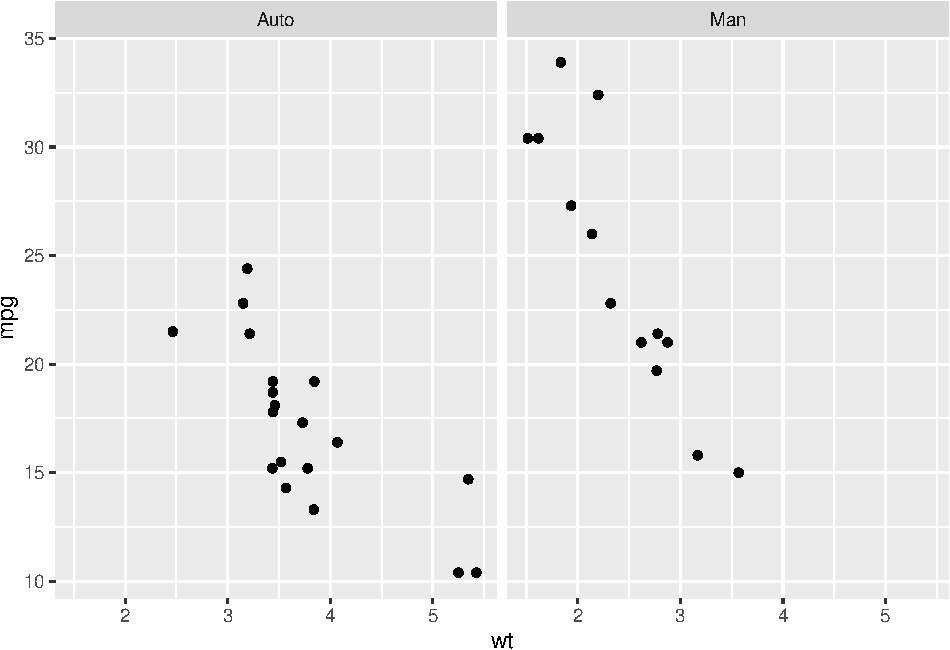
\includegraphics{nursing_741_files/figure-latex/unnamed-chunk-35-1.pdf}

\section{Sorting data}\label{sorting-data}

Sorting rows in a data fram is a common activity. However, in Base R
this is called ``ordering'' because of the function used to ``order''
the data. Let's say we want to sort or ``order'' the mtcars data frame
such that the row with the lowest mpg value is listed first and the row
with the highest mpg value is listed last. First, look at the
\textbf{order} function's output. What are those numbers ?

\begin{Shaded}
\begin{Highlighting}[]
\KeywordTok{order}\NormalTok{(mtcars}\OperatorTok{$}\NormalTok{mpg)}
\end{Highlighting}
\end{Shaded}

\begin{verbatim}
##  [1] 15 16 24  7 17 31 14 23 22 29 12 13 11  6  5 10 25 30  1  2  4 32 21
## [24]  3  9  8 27 26 19 28 18 20
\end{verbatim}

Oh, so they are row numbers corresponding to rows in mtcars. Row 15 has
the car with the lowest mpg. Row 16 corresponds to the car with the next
lowest mpg and so on. So we can use this information to order our
dataframe accordingly:

\begin{Shaded}
\begin{Highlighting}[]
\NormalTok{mtcars[}\KeywordTok{order}\NormalTok{(mtcars}\OperatorTok{$}\NormalTok{mpg),]}
\end{Highlighting}
\end{Shaded}

\begin{verbatim}
##                      mpg cyl  disp  hp drat    wt  qsec vs   am gear carb
## Cadillac Fleetwood  10.4   8 472.0 205 2.93 5.250 17.98  0 Auto    3    4
## Lincoln Continental 10.4   8 460.0 215 3.00 5.424 17.82  0 Auto    3    4
## Camaro Z28          13.3   8 350.0 245 3.73 3.840 15.41  0 Auto    3    4
## Duster 360          14.3   8 360.0 245 3.21 3.570 15.84  0 Auto    3    4
## Chrysler Imperial   14.7   8 440.0 230 3.23 5.345 17.42  0 Auto    3    4
## Maserati Bora       15.0   8 301.0 335 3.54 3.570 14.60  0  Man    5    8
## Merc 450SLC         15.2   8 275.8 180 3.07 3.780 18.00  0 Auto    3    3
## AMC Javelin         15.2   8 304.0 150 3.15 3.435 17.30  0 Auto    3    2
## Dodge Challenger    15.5   8 318.0 150 2.76 3.520 16.87  0 Auto    3    2
## Ford Pantera L      15.8   8 351.0 264 4.22 3.170 14.50  0  Man    5    4
## Merc 450SE          16.4   8 275.8 180 3.07 4.070 17.40  0 Auto    3    3
## Merc 450SL          17.3   8 275.8 180 3.07 3.730 17.60  0 Auto    3    3
## Merc 280C           17.8   6 167.6 123 3.92 3.440 18.90  1 Auto    4    4
## Valiant             18.1   6 225.0 105 2.76 3.460 20.22  1 Auto    3    1
## Hornet Sportabout   18.7   8 360.0 175 3.15 3.440 17.02  0 Auto    3    2
## Merc 280            19.2   6 167.6 123 3.92 3.440 18.30  1 Auto    4    4
## Pontiac Firebird    19.2   8 400.0 175 3.08 3.845 17.05  0 Auto    3    2
## Ferrari Dino        19.7   6 145.0 175 3.62 2.770 15.50  0  Man    5    6
## Mazda RX4           21.0   6 160.0 110 3.90 2.620 16.46  0  Man    4    4
## Mazda RX4 Wag       21.0   6 160.0 110 3.90 2.875 17.02  0  Man    4    4
## Hornet 4 Drive      21.4   6 258.0 110 3.08 3.215 19.44  1 Auto    3    1
## Volvo 142E          21.4   4 121.0 109 4.11 2.780 18.60  1  Man    4    2
## Toyota Corona       21.5   4 120.1  97 3.70 2.465 20.01  1 Auto    3    1
## Datsun 710          22.8   4 108.0  93 3.85 2.320 18.61  1  Man    4    1
## Merc 230            22.8   4 140.8  95 3.92 3.150 22.90  1 Auto    4    2
## Merc 240D           24.4   4 146.7  62 3.69 3.190 20.00  1 Auto    4    2
## Porsche 914-2       26.0   4 120.3  91 4.43 2.140 16.70  0  Man    5    2
## Fiat X1-9           27.3   4  79.0  66 4.08 1.935 18.90  1  Man    4    1
## Honda Civic         30.4   4  75.7  52 4.93 1.615 18.52  1  Man    4    2
## Lotus Europa        30.4   4  95.1 113 3.77 1.513 16.90  1  Man    5    2
## Fiat 128            32.4   4  78.7  66 4.08 2.200 19.47  1  Man    4    1
## Toyota Corolla      33.9   4  71.1  65 4.22 1.835 19.90  1  Man    4    1
\end{verbatim}

To invert the sense of the order use the \textbf{rev} function. We'll
also use the head function to list only the first 5 rows of the result.
Note that in base R, using composite functions is welcomed although you
will find out that this is not a value in the tidyverse. For math
people, using a composite function is natural which, in large part, is
why R embraced that approach early on.

\begin{Shaded}
\begin{Highlighting}[]
\KeywordTok{head}\NormalTok{(mtcars[}\KeywordTok{rev}\NormalTok{(}\KeywordTok{order}\NormalTok{(mtcars}\OperatorTok{$}\NormalTok{mpg)),])}
\end{Highlighting}
\end{Shaded}

\begin{verbatim}
##                 mpg cyl  disp  hp drat    wt  qsec vs  am gear carb
## Toyota Corolla 33.9   4  71.1  65 4.22 1.835 19.90  1 Man    4    1
## Fiat 128       32.4   4  78.7  66 4.08 2.200 19.47  1 Man    4    1
## Lotus Europa   30.4   4  95.1 113 3.77 1.513 16.90  1 Man    5    2
## Honda Civic    30.4   4  75.7  52 4.93 1.615 18.52  1 Man    4    2
## Fiat X1-9      27.3   4  79.0  66 4.08 1.935 18.90  1 Man    4    1
## Porsche 914-2  26.0   4 120.3  91 4.43 2.140 16.70  0 Man    5    2
\end{verbatim}

\chapter{Literature}\label{literature}

Here is a review of existing methods.

\chapter{Methods}\label{methods}

We describe our methods in this chapter.

\bibliography{book.bib,packages.bib}


\end{document}
